\chapter{Implementace} 
\section{Architektura}
V tomto frameworku rozlišujeme klientskou a serverou část. Serverová část generuje data pro klienta a tímto způsobem ovlivňuje ovládací prvky, které klientská část aplikace zobrazuje uživateli. Diagram nasazení na obrázku \ref{img:deploymentFrameworkDiagram} zachycuje použití frameworku. Serverová část frameworku je nasazena na klientovi a je schopná generovat definice formulářů s použitím frameworku AspectFaces \cite{aspectFaces}. Tyto definice jsou převedeny na model, který je možné upravit a odeslat klientovi. Aby byla serverová část plně funkční je potřeba nasadit aplikaci, v které je využívána na Java EE aplikační server. Nicméně v případě využití pouze staticky generovaných definic, lze aplikaci nasadit na libovolný aplikační server, který bude poskytovat klientům definice kompatibilní s definici poskytovanými při dynamickém generování. Specifikace formuláře, je poté zaslána na klienta, který ji interpretuje za použítí klientské částy zvané AFSwinx. Tato část využívá i serverovou část a to z důvodu kompatibilnosti objektů a jejich vlastností. Přidání do projektu lze provést tak, že se do adresáři s knihovnami vloží přeložený jar soubor, či se přidá projekt jako Maven závislost. V současné době není framework k dispozici v centrálním repositáři, je tedy potřeba stáhnout aktuální verzi a zkompilovat ji do lokálního repositáře.  
\subsection{Server}
Jak již bylo zmíňěno, tak server využívá ke generování serverou část frameworku nazvanou AFRest. Na obrázku \ref{img:serverSide} jsou zobrazeny třídy a balíčky, které tato část využívá. Jsou zde výčtové typy, které určují podporované komponenty a jejich vlastnosti, dále objekty zodpovědné za informace o volbě layoutu a objekty nesoucí informace o definicích, na základě kterých budou sestaveny formuláře či tabulky klientem a samozřejmě třídy zodpovědné za inspekci dat. Framework doplňuje do AspectFaces několik anotací, které lze využít při generování definic. Jsou to následující anotace:
\begin{enumerate}
\item @UIWidgeType - tato anotace určuje typ widgetu, který se použije do xml šablon, které se používají při generování definic je propagován jako proměnná s názvem widgetType
\item @UILayout - tato anotace definuje layout na dané proměnné. Lze specifikovat typ layoutu, jeho orientace a pozice popisu prvku. Do xml šablon jsou tyto hodnoty propagovány jako layout, layoutOrientation a labelPossition. 
\end{enumerate}
Výše zmíněné anotace akceptují pouze hodnoty z výčtových typů v balíčku common. V případě typu komponenty nebo-li widgetType přijímá anotace hodnoty ze třídy SupportedWidgets a v případě anotace určující layout lze vložit pouze hodnoty z výčtových typů LayoutDefinitions, LayoutOrientation a LabelPosition. Hlavní výhodou tohoto řešení, je typová kontrola a jistota, že klient obdrží od serveru pouze takové hodnoty, s kterými je schopný pracovat. Stejným principem jsou řešeny validace a proměnné, které definují vlastnosti jednotlových komponent. 

\subsubsection{Generování modelu}
Výsledkem inspekce objektu je model, který nese informace potřebné k tomu, aby klient mohl sestavit formulář či tabulku a byl do těchto komponent schopný vložit data získaná ze serveru. Na obrázku \ref{img:metaModelFinal} je konečná podoba modelu, který je vytvořen k tomuto účelu. Model je výsledkem hledání analytických tříd z doménového modelu na obrázku \ref{img:metadataMode}. Tento model již byl posán v analytické části, nicméně v této části je již model kompletní a proto zde budou uvedeny pouze změny oproti původnímu modelu. Proměnné, které nesou informace o layoutu, typu komponenty validátorech a jejich typech jsou výčtové typy. Jak již bylo zmíněno výhodou je typová bezpečnost a jednoznačnost vlastností, které framework podporuje. Model slouží také jako fásada, k nastavení dodatečných atributů. Jedním z těchto atributů je proměnná options ve třídě AFFieldInfo. Tato proměnná drží informace o možných hodnotách, které může komponenta nabývat. V současné verzi je tento atribut využit u komponent výběrového typu, mezi které patří například zaškrtávací políčka, či výběrová menu. Programátor specifikuje množinu těchto hodnot, v které klíč určuje hodnotu, jenž bude odeslána na server a text, který bude zobrazen uživateli je určen proměnnou value. Tyto možnosti nejsou generovány automaticky a v případě potřeby je musí programátor specifikovat ručně a to tak, že určí množinu dat a pole, ke kterému je přiřazeno. Třída AFMetaModelPack poskytuje zapouzdřuje způsob jakým se množina dat nastaví na konkrétní políčko a nabízí uživateli funkci, která je schopná nastavení provést na základě dat, zadaných uživatelem.

K dynamickému generování definic se využívá framework AspectFaces \cite{aspectFaces}, který umožňuje na základě mapování rozhodnout jaká komponenta bude použita pro konkrétní proměnnou dané třídy. Dále nabízí určení layoutu, který bude použit a samozřejmě určení mapovacího souboru. Tímto lze docílit mnoha různých transformací. Tento framework je potřeba nejprve nastavit, nicméně toto nastavení provede za vývojáře serverová část frameworku AFRest. Rozhranní AFRest z obrázku \ref{img:metaModelFinal} a jeho implementace AFRestGenerator provedou kompletní nastavení a spustí generování dat. Rozhranní umožňuje uživateli určit mapovací soubor a template, která bude použita. Mapování lze použít na všechny promměné obejktu, či může vývojář určit, které mapování se použije na konkrétní proměnnou. Ukázka mapování z frameworku AspectFaces je na znázorněna v ukázce zdrojových kódu \ref{code:xmlMapping}. Proměnná typu String se bude mapovat na vstupní textové pole, kterýé je definováno v structure/inputField.xml, v případě že se bude jednat o typ password, tak se bude proměnná typu String mapovat na vstupní textové pole typu, které místo vepsaných znaků zobrazuje zástupné znaky, komponenta je definována v structure/inputPassword.xml. Typ Address, což je neprimitivní datový typ se bude mapovat na entitní typ, jehož definice je v structure/entity.xml.
\begin{lstlisting}[caption=Ukázka mapování proměnných na komponenty,
  label={code:xmlMapping}]
<mapping>
	<type>String</type>
	<default tag="structure/inputField.xml" maxLength="255"/>
	<condition expression="${type == 'password'}" tag="structure/inputPassword.xml" />
</mapping>
<mapping>
	<type>Address</type>
	<default tag="structure/entity.xml" />
</mapping>
\end{lstlisting}
Mapování tedy určí soubor s komponentou, který bude reprezentovat aktuální proměnnou. Soubor s definicí komponenty, je pak dále využit k finálnímu definici proměnné. Ukázka vstupního textového pole je v ukázce zdrojových kódu \ref{code:xmlInputField}. Komponenta je v kořenovém elementu widget. Jelikož se jedná pouze o fragment xml, který je použit ke složení celé definice, jenž je uvedena v příloze v ukázce zdrojových kódů \ref{code:xmlCompleteDefinition}, tak zde není uvedena deklarace XML \cite{xml}. Ve výsledném XML již však deklarace již uvedena je. Popis jednotlivých uzlů je v tabulce \ref{table:xmlComponentAttributes}.
\begin{lstlisting}[caption=Ukázka definice komponenty,
  label={code:xmlInputField}]
<widget>
	<widgetType>textField</widgetType>
	<fieldName>$field$</fieldName>
	<label>$label$</label>
	<validations>
		<required>$required$</required>
		<minLength>$minLength$</minLength>
		<maxLength>$maxLength$</maxLength>
	</validations>
	<fieldLayout>
		<layoutOrientation>$layoutOrientation$</layoutOrientation>
		<labelPossition>$labelPossition$</labelPossition>
		<layout>$layout$</layout>
	</fieldLayout>
</widget>
\end{lstlisting}
Knihovna AspectFaces umožňuje určovat způsob jakým bude prováděna inspekce. Tento způsob se určuje v šablonách. K optimálnímu využití je nejvýhodnější použít způsob, při kterém je provedena inspekce všech proměnných, které mají definováno mapování. V případě jednoduchých datových typů je vše v pořádku, nicméně knihovna neobsahovala nativní podporu pro neprimitivní datové typu, v případě že byla použita inspekce, která by nevyužívala JSF. Z tohoto důvodu je důležité, aby se všechny neprimitivní datové typy mapovali na entity.xml, která je znázorněna v části zdrojového kódu \ref{code:xmlEntity}. Framework totiž pro všechny tyto entity provede inspekci znovu a následně části sestaví sestaví a vznikne tak kompletní definice. V tomto bodě, lze určit mapování a šablony, které se mají při rekurzivní inspekci použít. Framework AspectFaces byl proto doplněn o proměnné, které umí vrátit kanoický název třídy a na základě tohoto názvu lze provést nad touto třídou inspekci. Jak je patrné z výsledné definice, tak každý uzel má svého rodiče. Na základě rodiče lze určit jednoznačně určit kam uzel patří. Tato vlastnost umožňuje provádět inspekci i nad třídami, které mají více proměnných stejného datového typu. Klient totiž potřebuje znát strukturu objektu, aby ho mohl zpětně sestavit a odeslat zpět na server, který objekt přijme. Znalost struktury klient taktéž vyžaduje v případě získávání dat.
\begin{lstlisting}[caption=Ukázka definice neprimitvního datového typu,
  label={code:xmlEntity}]
<entityClass>
	<entityFieldType>$DataTypeFullClassName$</entityFieldType>
	<fieldName>$fieldName$</fieldName>
</entityClass>
\end{lstlisting}
\subsubsection{Použití}
Aby byl klient schopný získat definice dat, tak musí serverová strana poskytovat zdroj těchto definic. V tomto zdroji server využije serverovou část frameworku ke generování dat. Použití je přímočaré a ukázka zdroje je zobrazena na v části zdrojového kódu \ref{code:serverDefinition}. Nejprve je vytvořena instance třídy AFrestGenerator, která umožňuje generování dat, jenž jsou následně odeslány klientovi. Generátor nastaví framework AspectFaces automaticky, nicméně očekává, že bude framework AspectFaces, použit. K správnému použití je potřeba, aby we WEB-INF byly konfigurační soubory a aby existovali mapovací soubory a definice komponent. V tomto případě využije implicitního nastavení pro mapování i šablony. Bude použito mapování v souboru structure.config.xml a šablona v template/structure.xml. Tyto ukázkové soubory jsou poskytovány spolu s frameworkem.

\begin{lstlisting}[caption={Ukázka zdroje, sloužícího k vygenerování definice třídy Country},
  label={code:serverDefinition}]
@GET
@Path("/definition")
@Produces({MediaType.APPLICATION_JSON})
@Consumes({MediaType.APPLICATION_JSON})
@RolesAllowed({"admin"})
public Response getResources(@javax.ws.rs.core.Context HttpServletRequest request) {
	try {
		AFRest afRest = new AFRestGenerator(request.getSession().getServletContext());
		AFMetaModelPack data = afRest.generateSkeleton(Country.class.getCanonicalName());
		return Response.status(Response.Status.OK).entity(data).build();
	} catch (MetamodelException e) {
		return Response.status(Response.Status.INTERNAL_SERVER_ERROR).build();
	}
}
\end{lstlisting}
Zdroj poskytuje definice dat. V případě, že klient požaduje data do vygenerované definice, tak je potřeba poskytnout klientovi objekt stejného typu, nad kterým byla prováděna definice, nebo objekt se stejnými proměnnými a datovými typy. V tomto případě třídu Country. Klientská strana nerozlišuje datový typ obdrženého objektu, avšak očekává, že objekt bude mít určité proměnné, ke kterým se budou vázat specifické validace. V některých případech je žádoucí, aby se na úrovni business a view nepracovalo s databázovou entitou, ale s jejím mapovacím objektem. V části zdrojových kódu \ref{code:serverData} je příklad získání dat do již vygenerovaného formuláře či tabulky. Zdroj využije EJB managera CountryManager k získání konkértní instace třídy Country z databáze. Tuto instanci vrátí klientovi. Tento zdroj nemá žádnou vazbu na předchozí zdroj, který generoval definice. Vývojář tedy v případě použítí frameworku nemusí měnit stávající implementaci, pokud již nějaká existuje. Stejně tak nemá použití frameworku dopad ne klienty, kteří již používají webové API serveru. Zodpovědnost za správnou interpretaci dat je na klientské straně.
\begin{lstlisting}[caption=Zdroj poskytující konrétní instanci třídy Country,
  label={code:serverData}]
@GET
@Path("/{id}")
@Produces({MediaType.APPLICATION_JSON})
@Consumes({MediaType.APPLICATION_JSON})
public Response getCountry(@PathParam("id") int id) {
	try {
		CountryManager<Country> countryManager = getCountryManager();
		Country country = countryManager.findById(id);
		return Response.status(Response.Status.OK).entity(country).build();
	} catch (BusinessException e) {
		return Response.status(Response.Status.BAD_REQUEST).build();
	} catch (NamingException e) {
		return Response.status(Response.Status.INTERNAL_SERVER_ERROR).build();
	}
}
\end{lstlisting}

\begin{table}[width=\linewidth]
\begin{center}
\caption{Uzly XML, které definují strukturu dat}
\label{table:xmlComponentAttributes}
\begin{tabular}{|p{7cm}|p{7cm}|}
\hline
\textbf{Uzel} & \textbf{Popis} \\
\hline
widget & 
Typ komponenty. Určuje jak komponentu bude klient interpretovat.\\
\hline
fieldName &
Název aktuální proměnné, kterou komponenta zastupuje.\\
\hline
Label &
Popis komponenty, který bude zobrazen uživateli. \\
\hline
validations &
Validace, které bude umět komponenta ověřit. \\
\hline
fieldLayout&
Popis layoutu, který bude na komponentě použit. \\
\hline
\end{tabular}
\end{center}
\end{table}


\subsection{Klient}
Klientská část aplikace, využívá klientskou část frameworku ke generování formulářů či tabulek. Definice a data získává ze server. Referenční implementace je napsána pro standalone aplikace na platformě Java SE s využitím technologie Swing. Integrace frameworku do klientské aplikace je možná dvěmi způsoby. Prvním z nich je vložení knihovny do složky lib a druhým je přidání Maven závislosti. 
\subsubsection{Komponenty}
Klientská část umožňuje generovat tabulky nebo formuláře. Tyto celky označujeme jako komponenty. V případě formuláře se tato komponenta skládá z dalších aktivních ovládacích prvků. Komponenty jsou oděděny z třídy AFSwinxTopLevelComponent, která implementuje rozhraní AFSwinxInteraction, jenž vynucuje implementovat metody k získání modelu, dat a k jejich odeslání zpět na server. Součáští je také validace dat. Mimo tohoto rozhraní používá implementuje třída ještě rozhranní ComponentResealization. Toto rozhranní je využito k zpětnému získání dat z komponent. Aby bylo možné přidávat komponenty do již existující aplikace, tak tato komponenta ještě dědí od třídy JPanel, což zajistí, že výslednou komponentu lze přidat na jakékoliv místo ve stávající Swingové aplikaci. Vývojář může nad takto generovanými komponentami provádět operace. V případě odeslání dat na server, lze tuto akci vyvolat metodou sendData. Komponenta již sama provede validaci dat, sestavení dat a jejich odeslání.

Při návrhu jsem se zaměřil i na použitelnost, neboť je potřeba aby framework umožňoval dodatečná nastavení, nicméně pokud se vývojář bude s frameworkem učit, tak je pravděpodobné, že bude chtít vytvořit první prototyp, aby si vyzkoušel funkčnost. Z tohoto důvodu byla zavedena třída AFSwinx, která slouží jako správce komponent. Umožňuje komponenty vytvářet, přidávat, mazat nastavovat globální skin a lokalizace. Důležitou součástí je i získání již sestavené komponenty. Každá komponenta je jednoznačně určena svým identifikátorem, který si vývojář zvolí. Na základě tohoto identifikátoru je zaregistrována a lze k ní získat přístup a provádět nad ní operace. Vzhled jednotlivých prvků v komponentě již není možné po vygenerování měnit. Skiny a lokalizace musí být tedy nastaveny před samotným vygenerováním. Také je potřeba určit způsoby připojení ke zdrojům a jejich URI. Proces vytváření komponent vyžaduje několik operací, které na sebe navazují. V případě že by byl tento proces ponechán na vývojáři, tak by byl framework nepoužitelný. Z tohoto důvodu poskytuje třída AFSwinx buildery pro tabulky a formuláře, které komponenty sestaví, vloží do nich data a vývojáři vrátí výsledný JPanel. Typ komponenty určuje vývojář a buildery umí vytvořit formulář či tabulku na základě jedné definice. V případě tabulky je možné ještě provést dodatečné nastavení. Jedná se o automatické nastavení šírky sloupečků a automatické nastavení velikosti tabulky. Ukázka vytvoření formuláře je zobrazena v části zdrojových kódu \ref{code:formGeneration}. Nejprve je potřeba získat instanci builderu, který bude použit. Typ builderu určí zdali bude vytvořena tabulka či formulář. V tomto konkrétním případě bude vytvořen formulář. Metamodel získává klient ze serveru. Framework zapouzdřuje způsob získání dat, vývojář tedy musí definovat zdroje. Jednou z možností je specifikovat zdroje jako samostatné objekty, druhou možností je využít XML. V případě použití XML souboru musí být uveden soubor a identifikátor připojení. Tyto vlastnosti jsou nastaveny builderu pomocí metody initBuilder, která očekává identifikátor formuláře, soubor se specifikací připojení a identifikátor připojení. Builder má samozřejmě několik přetížených metod initBuilder. Tímto lze docílit různých způsobů počátečního nastavení. Metoda buildComponent již postaví vygeneruje výsledný formulář. Pokud se při generování vyskytne chyba, pak je vyhozena vyjímka AFSwinxBuildException. Je na vývojáři jak vyjímku zpracuje. V ukázce je zobrazen dialog s chybovou hláškou.

\begin{lstlisting}[caption={Generování formuláře na klientovi},
  label={code:formGeneration}]
File connectionFile =
	new File(getClass().getClassLoader().getResource("connection.xml").getFile());
	try {
		AFSwinxForm form =
			AFSwinx.getInstance().getFormBuilder()
			.initBuilder("loginForm", connectionFile, "loginFormConnection")
			.buildComponent();
	}catch (AFSwinxBuildException e) {
		getDialogs().failed("afswinx.build.title.failed", "afswinx.build.text.failed", e.getMessage());
	}
\end{lstlisting}

\section{Přenos modelu server klient a generování komponent}
Model na jehož základě jsou generovány komponenty je přenášen ze serveru na klienta. Klient musí tento model správně zpracovat a interpretovat. Nejprve je však potřeba model získat. Pro přenos modelu je použit protokol HTTP či HTTPS. Klientská strana poskytuje vývojáři nativní podporu k získání dat ze serveru. K tomuto účelu je využit framework HttpComponents \cite{apacheHttp}, který poskytuje předpřipravené komponenty, jenž lze využít k vytváření HTTP či HTTPS požadavků. Použitím této komponenty zjednoduší použití našeho frameworku, neboť vývojář nemusí ztrácet čas vytvářením tříd, které by byly schopné získat data ze serveru. Bohužel použití má i nevýhody. Vývojář nemůže ovlivnit implementaci toho, jak jsou data získána, pouze může ovlivnit způsob a to specifikací zdrojů a způsobů připojení. Z tohoto důvodu nabízí framework možnost specifikovat zdroje ve formátu XML s podporou EL. K získání modelu je potřeba mít definovaný zdroj v uzlu metamodel. Uzel se specifikací konkrétních dat a umístění kam data odeslat je nepovinný. Parsování pomocí DOM parseru je však provedeno nad všemi uzly konkrétního připojení a výsledkem je třída AFSwinxConnectionPack, které má reference na konkrétní připojení reprzentovanou třídou AFSwinxConnection. Ukázka je na obrázku \ref{img:connectionPack}. 	Mimo adresy, portu a protokolu lze specifikovat i hlavičku a v případě zabezpečení zdroje autorizaci k tomuto zdroji.

\begin{figure}[h!]
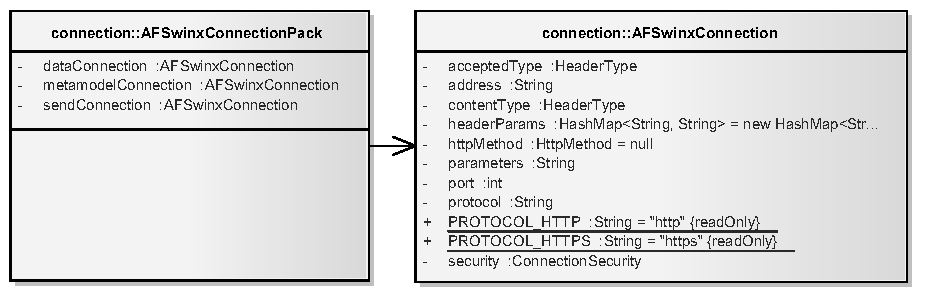
\includegraphics{images/connectionPack}
\caption{Třídy zodpovědné za specifikaci zdrojů a způsobu připojení.}
\label{img:connectionPack}
\end{figure}

\subsection{Generování komponent}
Vývojář na základě builderu určí jaká komponenta se bude generovat. Sekvenční diagram je na obrázku \ref{img:sdDiagram}. Z diagramu je patrné, že builder nejprve získá model ze serveru na základě specifikace zdroje, který mu byl předán během inicializace. Od serveru získá klient třídy reprezentující metamodel. Tento metamodel byl již popsán a je na obrázku \ref{img:metaModelFinal}. Klient nyní začne rekurzivně vytvářet již konkrétní aktivní prvky. Pro každou proměnnou objektu, bude vygenerován widget. Pokud se jedná o neprimitivní datový typ, tak se k příslušnému typu vyhledá jeho reprezentace v metamodelu a generování bude pokračovat tímto objektem. Takovýto přístup zajišťuje zachování pořadí proměnných. Pořadí proměnných lze měnit na serverové straně, nikoliv na klientovi. Typ aktivního prvku určuje atribut widgetType, který je součástí každého popisu konkrétní proměnné. Formulářový builder si nechá vytvořit od tovární třídy WidgetBuilderFactory, která je zodpovědná za vytváření konkrétního builderu, builder jenž je schopný vytvořit požadovaný aktivní prvek. Tento builder vrátí již konkrétní komponenty jako jsou například vstupní textová pole, zaškrtávací políčka a další, před kompletním generováním aktivního prvku lze nastavit jazykové lokalizace a skin. Tyto aktivní komponenty jsou zapouzdřeny v objektu AFSwinxPanel. Důvodem je, že tento panel již zohledňuje layout dané komponenty a mimo aktivní prvek obsahuje i popis, placeholder určený k zobrazení validační hlášky a všechny validace, které musí být nad tímto prvek vykonány. Panel si také udržuje jednoznačný identifikátor v rámci formuláře, na základě kterého lze poté určit jakou proměnnou prvek reprezentuje a její umístění v hiearchii tříd. Panel je následně přidán do dalšího panelu, který udržuje všechny prvky formuláře. V rámci tohoto formulářového panelu jsou také zohledněny layouty a uspořádání komponent. V tomto bodě je formulář sestaven a již nad ním lze provádět validace, či je možné formulář odeslat zpět na server. Nyní je potřeba rozhodnout zdali by měli být ve formuláři zobrazeny data či nikoliv. Formulářový builder vyhodnotí, zdali má naplnit formulář daty a to na základě specifikovaných zdrojů. Pokud byl zdroj s daty specifikován, pak jsou data získána a automaticky vložena do komponenty, jinak se formulář jíž nemodifikuje a práce builderu je ukončena.

\subsubsection{Vkládání dat do komponenty}
Data vkládá do komponenty builder vytváření této komponenty. Komponenta, kterou builder vytváří disponuje funkcionalitou, která ji umožní získat data ze serveru. O datovém objektu, který server poskytuje nemá komponenta předem žádné informace. Proto je tento objekt po obdržení převeden na třídu AFDataPack. Hiearichie je zobrazena na obrázku \ref{img:dataPack}. 
Klíč určuje umístění proměnné v hiearchii. V klíči je použita standardní tečková notace. Například mějme třídu Person, která má referenci na třídu Address přes proměnou myAdress a ve třídě Address je textová proměnná city. Pokud je třída Person první v hiearchii, tak je nahrazena zástupnou hodnotou root. Klíč k proměnné city je pak následující: root.myAdress.city. Stejným způsobem byly vygenerovány klíče pro konkrétní komponenty formuláře, jenž byly sestaveny na základě metadat. Formulář či tabulka mají tedy komponenty, které mají klíče kompatibilní s klíči vygenerovanými z obdržených dat. Lze je tedy spolu spárovat. Problémem však je, že každá z komponent je jiná a byla sestavena specifickým builderem. Nicméně builder zná tento způsob a proto mu byla přidána funkcionalita, na základě které lze upravit současný model a vložit data do již existující komponenty. Typ builderu je určen na základě widgetType. Toto je proměnná, kterou disponují komponenty, jenž byly vytvořeny buildery. Data jsou vkládána do každé komponenty, která byla vytvořena.

\begin{figure}[h!]
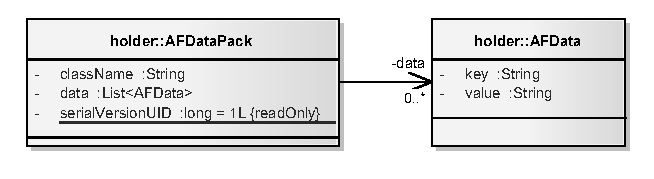
\includegraphics{images/dataPack}
\caption{Třídy, na které jsou převedena všechna data, jenž klient obdrží.}
\label{img:dataPack}
\end{figure}

\subsubsection{Widget builder}
V tabulce \ref{table:widgetBuilders} jsou popsány všechny widget buildery, které je možné použít. Všechny buildery mají společného předka. Abstraktní reprezentace buildera je znázorněna na obrázku \ref{img:abstractBuilder}. Konkrétní instance pak využívá společných metod, jenž jsou implementovány v jeho předkovi. Předek umí sestavit placeholder určený k zobrazení výsledku validací, popis ke každé komponentě, nastavit lokalizace, skiny včetně jejich aplikace a přidat validátory na pole. Tato abstraktní třída také umí vygenerovat dummy field, který je vytvořen pouze pokud komponenta dostala list hodnot jež může nabývat a současně není volba z tohoto listu povinná. Pak je zapotřebí udržovat informaci o tom, že uživatel volbu neučinil. Konkrétní prvky builderu z tabulky \ref{table:widgetBuilders} pak vytváří každý builder sám. 

\begin{lstlisting}[caption={Vytváření vstupního pole builderem.},
  label={code:textInputBuilder}]
public AFSwinxPanel buildComponent(AFFieldInfo field) throws IllegalArgumentException, AFSwinxBuildException {
	super.buildBase(field);
	// And input text field
	JTextField textField = new JTextField();
	customizeComponent(textField,field);
	layoutBuilder.addComponent(textField);
	coreComponent = textField;
	// Create panel which holds all necessary informations
	AFSwinxPanel afPanel =
		new AFSwinxPanel(field.getId(), field.getWidgetType(), textField, fieldLabel,
		message);
	// Build layout on that panel
	layoutBuilder.buildLayout(afPanel);
	// Add validations
	super.crateValidators(afPanel, field);
	return afPanel;
    }
\end{lstlisting}

Ukázka metody, která vygeneruje vstupní textové pole znázorněna v části zdrojových kódu \ref{code:textInputBuilder}. Nejprve jsou vytvořeny společné vlastnosti pro všechny buildery. Tyto vlastnosti vytváří abstraktní předek. Poté je na vytvořeno vstupné pole a na toto pole je aplikován skin. Komponenta je poté přidána do layout builderu. Následně je vytvořen AFSwinxPanel, jenž nese všechny nezbytné informace o aktuální komponentě. Tento panel je také přidán do layout builderu, který poté vytvoří konečné úspořádání komponent. Nakonec jsou v panelu registrovány všechny validátory, které se postupně spustí v případě odeslání dat, či v případě žádosti o zjištění validnosti formuláře.

\begin{lstlisting}[caption={Vložení dat do vstupního pole vytvořeného builderem.},
  label={code:textInputBuilderSetData}]
public void setData(AFSwinxPanel panel, AFData data) {
	if (panel.getDataHolder() != null && !panel.getDataHolder().isEmpty()) {
		JTextComponent textField = (JTextComponent) panel.getDataHolder().get(0);
		textField.setText(data.getValue());
	}
}
\end{lstlisting}

Jak již bylo zmíněno, tak builder tím, že zná způsob jakým byly komponenty vytvořeny, tak zná i způsob jakým jsou reprezentovány. V případě potřeby vložení dat do textového pole, je potřeba získat builder, který toto pole vytvořil a požádat ho o vložení dat. Ukázka je v části zdrojových kódů \ref{code:textInputBuilderSetData}. Builder nejprve ověří, zdali existují v panelu komponenty, pokud ano přetypuje je na konkrétní instance, které vytvářel. V tomto případě JTextComponent. Poté jim nastaví data specifickým způsobem pro danou komponentu.


\begin{table}[width=\linewidth]
\begin{center}
\caption{Widget buildery, kterými disponuje klient}
\label{table:widgetBuilders}
\begin{tabular}{|p{4cm}|p{3cm}|p{7cm}|}
\hline
\textbf{Builder} & \textbf{Typ widgetu} & \textbf{Popis} \\
\hline
DateBuilder & 
Calendar & Používá se při reprezentaci datového typu. Umožní uživateli zobrazit date picker, pomocí kterého lze vybrat datum.\\
\hline
DropDownMenuBuilder &
dropDownMenu & Menu, ze kterého lze vybrat jednu z několika voleb.\\
\hline
CheckBoxBuilder & checkBox &
Zaškrtávací políčko, či několik zaškrtávacích políček. Záleží zdali jsou uvedeny možnosti. V případě, že uvedeny nejsou vytvoří se jedno a pokud je zaškrtnuto tak je převedeno na hodnotu true.\\
\hline
InputBuilder & textField &
Builder pro textové pole. Není ničím omezeno.\\
\hline
LabelBuider & label &
Vypíše pouze textovou hodnotu. Do této komponenty nelze vkládat data či ji nijak upravovat. \\
\hline
NumberInputBuilder & numberField	 &
Vytvoří vstupní pole a přidá mu číselnou validaci. \\
\hline
OptionBuilder & option &
Vytvoří skupinu radiobuttonů, z které lze vybrat jednu hodnotu. \\
\hline
PasswordBuilder & password &
Vytvoří vstupní pole, v kterém jsou znaky nahrazeny zástupnými znaky. \\
\hline
TextAreaBuilder & textArea &
Vytvoří vstupní pole pro zadání velkého množství znaků. \\
\hline
\end{tabular}
\end{center}
\end{table}

\subsubsection{Skin}
Widget builder aplikuje na vygenerované komponenty skin. Skin lze nastavit již při získávání formulářového builderu. Skin určuje vzhled konkrétní komponenty. Pomocí skinu lze určit následující vlastnosti.
\begin{enumerate}
\item Barvu, typ fontu, výšku a šířku popisu, který je zobrazen u komponenty.
\item Barvu a typ fontu komponent.
\item Barvu a typ fontu validačních hlášek.
\item Šířku komponent. V případě textových polí i jejich výšku.
\end{enumerate}
Pokud není skin nastaven, tak je použita výchozí implementace, která je součástí frameworku. Vývojář si může definovat vlastní skin a to tak, že buď implementuje rozhranní Skin nebo využije dědičnost a překryje metody z třídy BaseSkin. Výhodou druhého přístupu je fakt, že vývojář může upravit pouze některé metody a nemusí implementovat všechny, které vyžaduje rozhraní.
\section{Přenos a generování dat klient server}
Formuláře a tabulky jsou vytvářeny k tomu, aby reprezentovali uživateli data v systému. Hlavním úkolem formulářů je také odeslání dat na server. Z předchozích sekcí je již zřejmé, že klientská část aplikace nedisponuje stejnými datovými objekty jako server, ale pouze popisem struktury daného objektu. Tato informace je však dostačující a lze na jejím základě vygenerovat data, která je schopný server přijmout. Přenost probíhá v několika krocích. Tyto kroky zachycuje sekvenční diagram na obrázku \ref{img:sdResealization}. Nejprve je zjištěno, zdali bylo při vytváření komponenty specifikován zdroj, na který se mají data odeslat. Před vygenerováním dat, která budou odeslána je provedena validace. V případě, že validace je úspěšná tak se začnou generovat data, která budou odeslána. K tomuto účelu slouží třída JSON builder, v případě že server očekává JSON. Framework nyní podporuje pouze JSON, nicméně návrh počítá s přidáním dalších datových builderů. Tyto buildery již neparsují data, která jsou uloženy v komponentě, za tuto činnost je zodpovědná konkrétní komponenta sama. Komponenta data parsuje z panelů, které si udržuje. Panel má jasně daný klíč, kterým lze určit umístění proměnné v původním objektu. Na základě tohoto klíče je vytvořen nový objekt. Klíč tedy určuje cestu. Pokud je v klíči znak tečky, tak to znamená, že je potřeba vyhledávat v již existující struktuře další potomky. Pokud již v klíči znak tečky není, tak to znamená, že jsme již na správném místě a objektu, který je reprezentován třídou AFDataHolder, jejíž ukázka je na obrázku \ref{img:afDataHolder},  bude přidána do jeho mapy další proměnná s hodnotou. Kromě klíče je potřeba znát i aktuální data v komponentě. Odobně jako při vkládání dat do komponenty je i při získávání dat využit konkrétní widget builder, který komponentu sestavil, neboť zná strukturu a způsob jak data z komponenty získat. JSON builder tedy dostane objekt, z kterého může data sestavit. K sestavení dat je využit framework GSON \cite{gson}. Když jsou již data sestavena tak je postačí odeslat na konkrétní zdroj, který byl specifikován při vytváření komponenty. Framework toto odeslání provede automaticky..

\begin{figure}[h!]
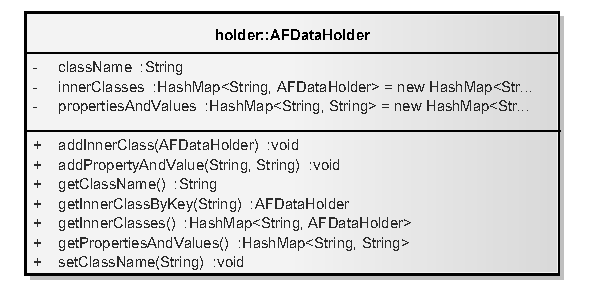
\includegraphics{images/AFDataHolder}
\caption{Třídy, které reprezentuje data ve formuláři. Na jejímž základě je sestaven objekt, který je odeslán na server.}
\label{img:afDataHolder}
\end{figure}

Pokud chce vývojář data odeslat například při kliknutí na tlačítko, tak musí provést pouze dva kroky. Nejprve musí získat konkrétní formulář který chce odeslat a poté nad ním zavolat akci sendData. Formulář lze získat z hlavní třídy AFSwinx na základě jeho identifikátoru kdekoliv v aplikaci. Žádné další akce nejsou potřeba. Mezi hlavní výhody patří snadná použitelnost formulářů a skutečnost, že je vývojář odstíněn od způsobu jakým se data odesílají. Nevýhodou je, že vývojář nemůže plně kontrolovat odeslání dat, či měnit implementaci odesílání a musí používat pouze metody, které mu framework nabízí.
\section{Lokalizace}
\section{Validace dat a vlastní validátory}
\section{Zabezpečení}
\section{Rozdíl mezi komponenty generovanými frameworkem a ručně psanými}

